\subsubsubsubsection{People carrier}
\begin{figure}[h]
\centering
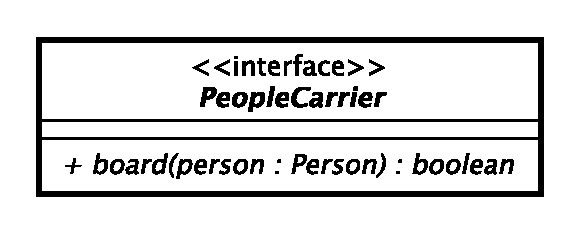
\includegraphics[scale=0.6,keepaspectratio]{images/solution/app/backend/people_carrier.eps}
\caption{\pActive::PeopleCarrier}
\label{fig:sd-app-people-carrier}
\end{figure}
\FloatBarrier
\begin{itemize}
  \item \textbf{\descr} \\
It represents an entity that carries people.
  \item \textbf{\ops}
  \begin{itemize}
    \item[+]  \texttt{\textit{board(person: Person): boolean}} \\
If the vehicle is not full the person become a passenger and the method 
returns \textit{true}. Otherwise the access to the vehicle is not granted and 
the method returns false.
  \end{itemize}
\end{itemize}
